\documentclass[12pt]{article} 
\usepackage[pdftex]{graphicx}
\usepackage{subfigure}
\usepackage{geometry, amsmath, amssymb, array, cite, caption, float}
\setlength{\parindent}{0pt} 
\setlength{\parskip}{2ex}
\bibliographystyle{unsrt} 
\begin{document} 
\title{Combined MRI and Optical Computed Tomography: Literature Review} 
\author{Ciara McErlean}
\date{23/1/13} 
\maketitle 
%\begin{abstract} This is a very short article. 
%\end{abstract} 
%\tableofcontents 

\section{Introduction}
\label{sec:intro}

Optical computed tomography reported before, as far back as 1983 (Ray and Semerjian, only 1 projection, sodium-seeded methane flame)\cite{ray1983laser} and again in 1990 (Kawata, algae)\cite{kawata1990laser}. Brown 1992 \cite{Brown:1992} has very similar setup to Gore and Sharpe. Used matching fluid (they call it clearing fluid) and cleared a sample of stained cochlea in 3BB:5MS. 600nm illumination to reduce scatter. 1.92mm radius imaged with resolution 16$\mu$m. But Brown is not referenced by either Gore or Sharpe. :(

\section{Theory}
\label{sec:theory}

\subsection{Radon Transform}
%Beers Law
%Radon transform and radon space

%Projections and sinograms leading to reconstruction techniques...

\subsection{Filtered Backprojection}
\label{subsec:FBP}

%Fourier Slice Theory

%Filtering, Hamm, Ram Lak, Shepp Logan

%Number of projections acquired affects image noise/blurriness. Don't need more than $180^{\circ}$.check

%Mention alternative, Algebraic Reconstruction Technique and other iterative methods. 


 \textit{Imaging with high resolution using this principle requires that the projection data are a direct result of the line integral of   the   parallel   rays   passing   through   the   sample.
} \cite{Wang:2006hy}

\textit{The optical images captured by the CCD are approximated as parallel projections throughout
 the specimen. A series of images at different views are then obtained by rotating the specimen.
 In such a way, the cross sections of the specimen can be independently reconstructed with the
 data on the corresponding rows of the CCD captured at sufcient different views.}\cite{Wang:2006hy}

\textit{ In fact, two assumptions are made to enable the conventional OPT to use the term of ‘projection’ and the reconstruction algorithm. First, the narrow cones of the light ray projected onto a CCD are assumed to be the strip integrals through the sample. Second, the axes of the light cones are taken to be parallel to each other. The two assumptions place severe constraints on the resolution of OPT imaging. In this paper, we present improved image-forming optics for OPT, with which the axes of the light cones are parallel to the optical axis of the optics. As a result, the parallel integral throughout a sample can be satisfied, and the second assumption mentioned above is relaxed. This method results in an improved spatial resolution, especially for the cross sections far from the optical axis}. \cite{Wang:2006hy}


Fourier slice theorem requirements, see Wang 2007 \cite{Wang:2007}

\subsection{Refractive index matching}

\subsection{Common artefacts}

Axis of rotation problems. Corrections suggested by many groups. Recently by Dong in 2012 \cite{Dong:2012}  discuss method.

%Ring artefacts are generated when a feature not associated with the dosimeter sample is present in the same place in all projections. A typical cause might be a bubble or scratch on the wall of the tank containing the matching liquid. (Directly from Doran 2008)

\newpage
\section{Dosimetry}
\label{sec:dos}
\subsection{Laser scanning configuration}
%\label{subsec:doshist}


One of the first reported optical computed tomography (OptCT) systems was developed in the area of gel dosimetry. Accurate 3-D measurement of dose delivery in radiotherapy is extremely important in developing safe treatment plans. Specialist polymer gels, such as BANG\textsuperscript{\textregistered} \cite{Maryanski:1996}, respond to irradiation with changes in optical attenuation and scattering properties.  This makes them ideal for measuring 3-D dose distributions. Previously the irradiated gels were measured by MRI and x-ray CT however, these are expensive imaging modalities. In 1996, Gore and Maryanski published the first system for scanning polymer gels using optical computed tomography. \cite{Gore:1999tg} In later comparisons, OptCT has been found to be more precise, have reduced noise and smoother line profiles than MRI for gel dosimetry. \cite{Oldham:2001gs}

Gore's system consisted of a  He-Ne laser source and large area photodiode detector (see Figure~\ref{fig:gore_setup}). Translate-rotate acquisition was employed whereby the sample was rotated and projection data  acquired  by the photodiode over $360^{\circ}$. The smaller the angular steps between projections, the more accurate the reconstruction. \cite{russ2002image} For a 2-D reconstruction, projections are acquired for multiple spots across a slice of the sample by translating the laser beam using mirrors. For 3-D information, the sample height  had to be manually adjusted and many 2-D slices acquired. This meant scanning an entire sample took  hours and lengthy scanning times are the chief disadvantage of the laser scanning method.  Accuracy of 5\% is reported and spatial resolution of 2mm, which is roughly the same as the laser beam width. \cite{Gore:1999tg}

The idea of OptCT scanning in dosimetry was quickly developed by other groups. Laser scanning set-ups were published in 1996 by Tarte \textit{et al.},  \cite{Tarte:2006} and Kelly \textit{et al.} [REF]
\textit{Can't find the paper 1996 Kelly references in 1998 \cite{Kelly:1998} Med Phys says it doesn't exist.}
Kelly \textit{et al.} claim to have independently developed their scanner which is very similar to that of Gore's. In in both Kelly's and Tarte's  scanners, the sample is rotated and translated using a stage whereas Gore used mirrors to translate the laser spot across the sample. 


A commercial laser scanning OptCT system, OCTOPUS\texttrademark by MGS Research, Inc.
(Madison, CT),  is an extension of Gore's original set-up with the addition of a platform capable of vertical movement for automated slice-selection. \cite{Islam:2003gs} For a number of years it was the only commercially available system and has been characterised by several groups. \cite{Xu:2003cc, Islam:2003gs, Xu:2004iv, Sakhalkar:2009hb} According to Oldham, characterisation of OptCT systems should include checks on geometric distortion, accuracy of reconstruction, scatter artefacts and reflection and refraction artefacts.\cite{Oldham:2004cj}


 

%Upgraded laser Oldham 2004b \cite{Oldham:2004bv} - field photodiode mounted on a scanning arm to maintain constant distance between laser and detector. Check Oldham 2006 \cite{Oldham:2007eu}

\begin{figure}[H]
\centering
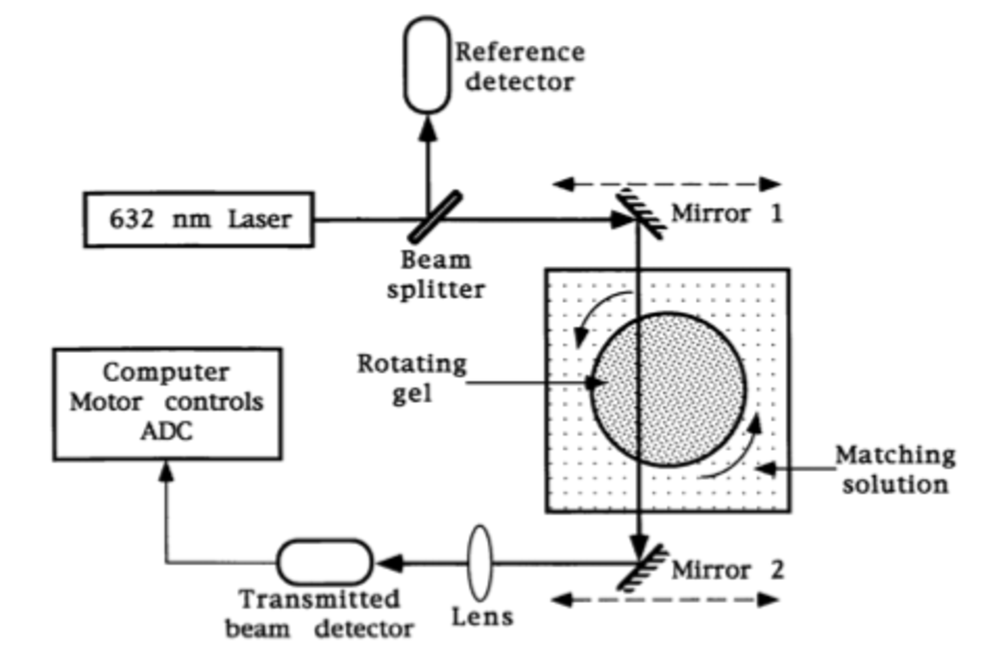
\includegraphics[scale=0.6]{Gore_setup.pdf}
\caption{A first generation,  Laser Scanning OptCT system developed by Gore. The sample is rotated and projections recorded at a number of angles. The  mirrors scan the laser beam across the sample but movement in the vertical direction is by manual adjustment only (figure from \cite{Gore:1999tg}). }
\label{fig:gore_setup}
\end{figure}


Laser scanning systems include a  beam splitter before the sample to create a reference beam. Dividing projections by the reference intensity  corrects for laser beam intensity fluctuations. \cite{Gore:1999tg}

Refraction and reflection at container walls are significant concerns for all configurations of dosimetry with OptCT. Generally, laser beams are incident on the gel container at a small angle, such as $5^{\circ}$, to avoid large reflection at the interface. In addition, the gel container is usually placed in a tank containing `matching fluid' with a refractive index close to that of the gel. This prevents significant refraction as the light passes into the gel. Doran found through ray tracing simulations that the refractive index of the walls of the matching tank and  gel container are not important compared to the gel and matching fluid. The optimum difference in refractive index between these two was calculated to be 0.0025 and not zero as originally thought.\cite{Doran:2001ee}

To maximise the dynamic range of the system, food dye is commonly added to the matching fluid so both the refractive index and optical density of the matching fluid and gel are very similar.\cite{Krstajic:2006kna} 




\subsection{Pixelated detector based systems}

In 1997 the first charge coupled device (CCD) camera based OptCT system was published by Tarte \textit{et al.} which employed an incoherent white light source and CCD camera detection. \cite{Tarte:2007} The advantage  of a pixelated detector based system  is that an entire 2-D projection can be imaged at once, potentially increasing the scanning speed by several  orders of magnitude depending on the data through-put rate. Tarte's system used a divergent light source and diffusing screen to measure optical density in a thin gel section (see Figure~\ref{fig:tarte_ccd_setup}). 
%For a very thin sample this adequate however, more sophisticated optics are required for bigger samples. \textbf{Does tarte reconstruct at all?}

\begin{figure}[H]
\centering
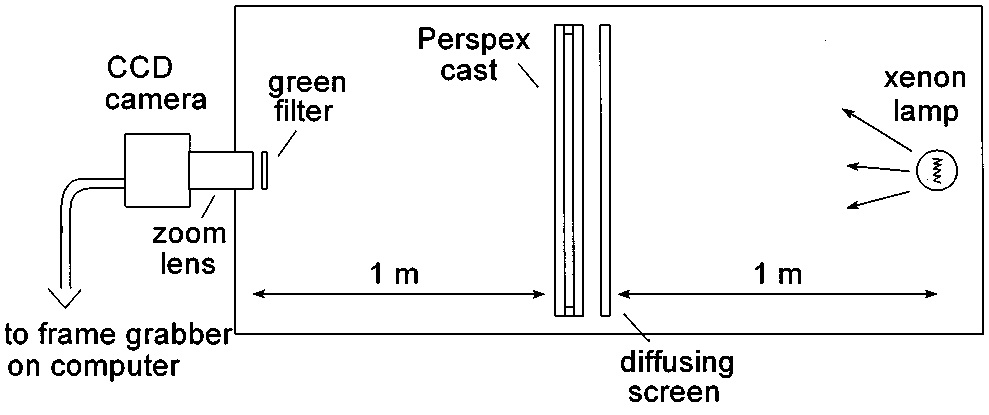
\includegraphics[scale=0.4]{Tarte_1997_ccdsetup.jpg}
\caption{Diagram of the first CCD-based  OptCT system, developed by Tarte \textit{et al.} It uses  divergent illumination from a white light source and CCD camera detection to record an entire 2D projection at once   (figure from \cite{Tarte:2007}). }
\label{fig:tarte_ccd_setup}
\end{figure}


The accuracy of Tarte's system  was checked by comparison with the standard measure of dosimetry, the parallel plate ionisation chamber. It was found to be on average within 3\% of the value from the ionisation chamber. \cite{Tarte:2007} A comparison between Tarte's laser scanning and CCD set-ups found that they had similar spatial resolutions. The CCD method had improved speed of acquistion but suffered from consistently worse SNR as a photodiode detector can collect many more photons per `pixel' than a CCD camera. \cite{Tarte:2007}

%The laser system 'pixel' is defined by the region illuminated by the laser spot while the photodiode has a much larger area than the spot, so it collects even photons which have diverged from a straight line. 

Advances in technology have meant that  high quality detectors are much more affordable. A cheaper alternative to very high quality CCD cameras is the CMOS (Complementary Metal-Oxide-Semiconductor) detector which has the potential for higher resolution and dynamic range. \cite{Doran:2008kh} Using a higher quality detector would improve many OptCT systems  in terms of scanning speed and reduced artefacts. \cite{Tarte:2007, Doran:2001ee}


\paragraph{Parallel beam configuration:} One method to reconstruct 3-D images with a CCD or CMOS detector is to create a broad parallel beam. This allows the use of parallel reconstruction algorithms, very similar to those used for x-ray CT. Each 2-D projection image recorded corresponds to one row for every slice in the 3-D reconstruction sinogram. \cite{Doran:2008kh}
Telecentric optics, in which the chief rays are parallel to the optical axis, are key in the design of this configuration. \cite{Walls:2005ja} Telecentric optics can be achieved either through a careful arrangement  of  a large converging lens before the sample and standard camera lens  \cite{Doran:2001ee} (see Figure~\ref{fig:doran_ccd_setup}) or through an expensive telecentric lens \cite{Sakhalkar:2008exa}. The process of forming a parallel beam results in non-uniformities in the lightfield. This is compensated for by subtracting a `correction' or `open lightfield', image which is a projection taken with no sample in the tank. \cite{Doran:2001ee}


\begin{figure}[H]
\centering
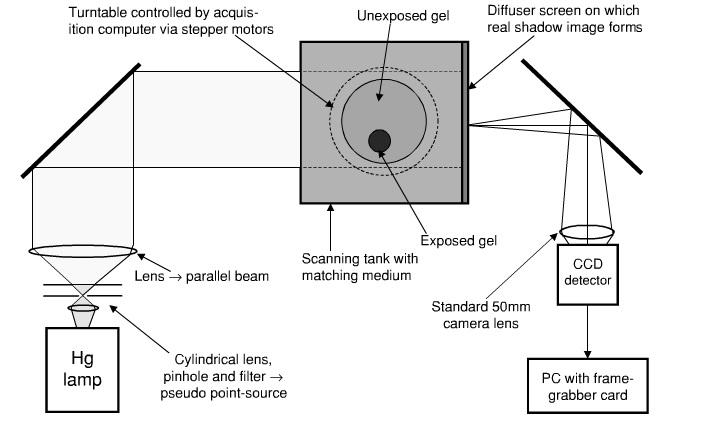
\includegraphics[scale=0.6]{Doran_2001_ccdsetup.jpg}
\caption{Diagram of a parallel beam  OptCT system, developed by Doran \textit{et al.} Telecentric optics create a parallel beam  (figure from \cite{Doran:2001ee}). }
\label{fig:doran_ccd_setup}
\end{figure}



Initial systems  suffered from `graininess' due to the unstable gain of cheap CCD cameras and granularity of the diffusing screen. \cite{Doran:2001ee}   Doran \textit{et al.} proposed some methods of correcting these problems. Oscillating the diffuser screen at high frequency 
``\,`smears' out the granularity'' while randomly horizontally displacing the CCD camera by a few pixels  between acquisitions can reduce the effect of `bad'  pixels.
 \cite{Doran:2001ee}
 The parallel configuration appears to be more susceptible to schlieren artefacts caused by refractive index inhomogeneities in the sample. \cite{Krstajic:2007hk}






\paragraph{Cone beam configuration:}
Wolodzko \textit{et al.} published the first cone beam OptCT system with CCD detection for gel dosimetry.\cite{Wolodzko:1999} One advantage of this configuration is the optics for producing a cone beam are much simpler than those for producing accurate parallel beams. \cite{Doran:2008kh} However, the reconstruction is computationally more complex. \cite{hsieh2003computed} A commercial cone-beam system, Vista\texttrademark by Modus Medical Devices Inc. (London, ON, Canada),  is available and reviewed recently by Olding \textit{et al.} \cite{Olding:2011eta}


\begin{figure}[H]
\centering
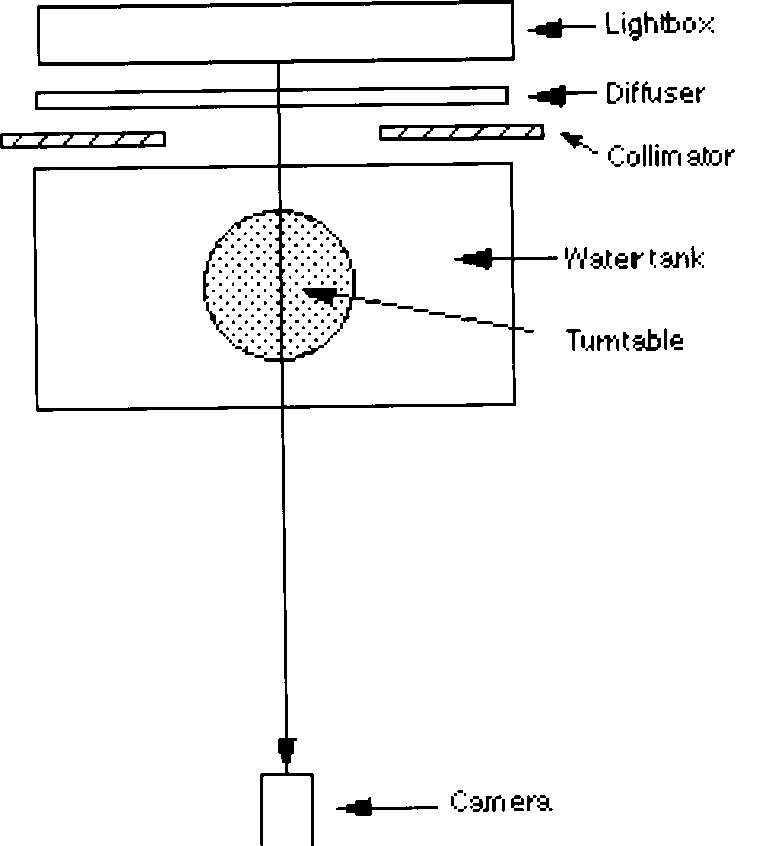
\includegraphics[scale=0.3]{Wolodzko_1999_conesetup.jpg}
\caption{Cone-beam CCD configuration (figure from \cite{Wolodzko:1999}).}
\end{figure}

When pixelated detectors are used, there appears to be more literature based on the parallel beam configuration than cone-beam. Although there has not been experimental comparison of the two Doran suggests that while cone-beam is usually somewhat cheaper due to simplified optics, modern parallel-beam systems have better scatter-rejection and may have fewer stray light problems. \cite{Doran:2008kh, Olding:2011eta, Thomas:2011eja}



 

 




%Refraction and reflection at container walls are significant concerns for all configuration of dosimetry with OptCT. These problems have been investigated with Mie theory modelling of light paths. Doran found through ray tracing simulations that the refractive index of the walls of the matching tank and  gel container are not important compared to the gel and matching fluid. The optimum difference in refractive index between these two was calculated to be 0.0025 and not zero as originally thought.\cite{Doran:2001ee} Another counter intuitive finding was that the ideal gel container wall thickness is not the thinnest possible but some median thickness which 

%Problems with vial walls misrepresentation due to refractive index mismatch. \cite{Doran:2001ee}

%Illumination is chosen based on the configuration used and the wavelength range which is optimum for dose measurement.  
%Stray light minimisation is very important in OptCT. Dark room, shield the illumination source. Interference filters. REF 
 

%Repeatability of experiments, have locking method for samples. REF
%Centre of rotation recovery, mostly post-processing. In theory section. 			

%\textit{The first is laser based and has several design considerations including minimisation of interference effects and stray light; scatter from optical components and the radiochromic gels themselves, reflection; dynamic range; wavelength selection; wall corrections plasma discharge from lasers; temperature changes; and the characterisation of detectors.A general disadvantage of scanners based on pixelated detectors together with a wide beam is the possible introduction of artefacts by refractive index inhomogeneities (schlieren). } from \cite{Doran:2008kh}







\newpage
\section{Tissue imaging}
\subsection{Optical Projection Tomography}

Another version of OptCT was  developed by Sharpe \textit{et al.} in the area of 3-D microscopy for gene expression studies. \cite{Sharpe:2002jp} Although this set-up in 2002 came after Gore's they are apparently independent and Sharpe named his technique Optical Projection Tomography (OPT).

Other techniques for 3-D microscopy include confocal microscopy which can image to a depth of about 1mm. \cite{Webb:1996} However, this is limited to fluorescent signals meaning many optical stains used routinely in histology would not work. Optical coherence tomography is another technique capable of micrometer-scale resolution. \cite{huang1993optical} However, its depth is limited to 2-3mm in tisse. Sharpe's OPT set-up could image much larger specimen, up to 15mm thick.  \cite{Sharpe:2002jp} OPT is a projection based tomography technique, as the name implies, which means mathematical reconstruction is required. The other techniques mentioned give tomographic images by sectioning. \cite{Sharpe:2003cm} \textbf{Discuss}

Sharpe's system includes a microscope to focus projections of a mouse embryo onto a camera imaging chip (CIC). Image-focusing optics are one difference between OPT and x-ray CT, which records shadows of the sample. Sharpe reports some impressive images (see Figure~\ref{fig:SharpeOPT}). Use of the microscope gives resolution of about 5-10$\mu$m meaning single-cell membranes, around 10$\mu$m thick, can be seen.\cite{Sharpe:2002jp} The axis of rotation is chosen so only half of the specimen is in focus at once which compensates for poor depth of focus. 

To reduce scattering and refraction within the specimen it was immersed in Murray's Clear, also known as BABBs (1:2 mixture of benzyl alcohol and benzyl benzoate). BABBs works as an optical clearing agent (OCA) which reduces refraction by replacing fluid in a specimen. The OCA is chosen with a refractive index close to that of the solid structures in the specimen. See Section~\ref{sec:clearing} for more detail on the clearing mechanism and possible agents. 
The result of clearing means that the light paths through the specimen can be approximated as parallel line integrals  making high resolution reconstruction through back projection possible.



\begin{figure}[H]
\centering
\subfigure[OPT setup]{\label{subfig:OPTsetup}
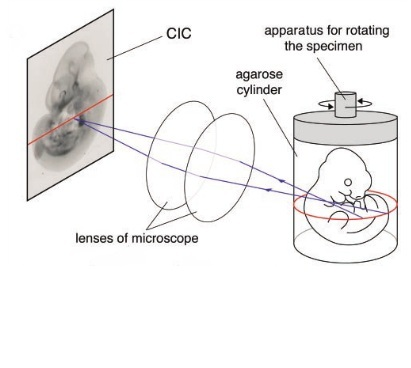
\includegraphics[width=0.6\textwidth]{Sharpe_2002_setup.jpg}}
\subfigure[Mouse images]{\label{subfig:OPTmouse}
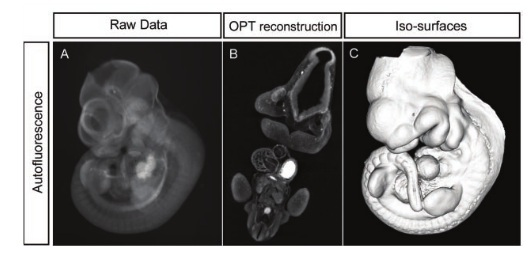
\includegraphics[scale=0.8]{Sharpe_2002_mouse.jpg}}
\caption{Part (a) shows the optical setup for the first OPT system by Sharpe. CIC indicates the camera imaging chip. A microscope is used to focus. The specimen is set in agarose gel for stability. Part (b) shows some sample images from OPT scanning of a mouse embryo. The iso-surface shows contours linking all regions above a certain intensity. Both figures are adapted from \cite{Sharpe:2002jp}.}
\label{fig:SharpeOPT}
\end{figure}




In 2005 Fauver reported a modified version of OPT capable of imaging single cell nuclei with 0.9$\mu$m resolution (see Figure~\ref{fig:fauver_setup}).\cite{Fauver:2005} The OPT microscope includes a rotation stage and  piezoelectrically driven objective lens. In a technique similar to Hausler \cite{hausler1972method} the objective lens is scanned axially to create an extended depth of field (DOF) image which is also known as a pseudoprojection. The extended DOF means features have the same focus from all angles, allowing high resolution reconstruction. However, this is not a truly quantitative technique, hence pseudo and not true projections are recorded. A high numerical aperture (NA) lens gives high resolution at the expense of low depth of field. If such high resolution is not required, low NA optics such as those used by Sharpe would be a more accurate way to generate  projections than scanning a high NA lens.\textbf{CHECK} 

%$180^{\circ}$ of data taken. Microcapillary, some cells injected into it. Rotation to sub-micron precision. Refractive index matching to 0.02.



\begin{figure}[H]
\centering
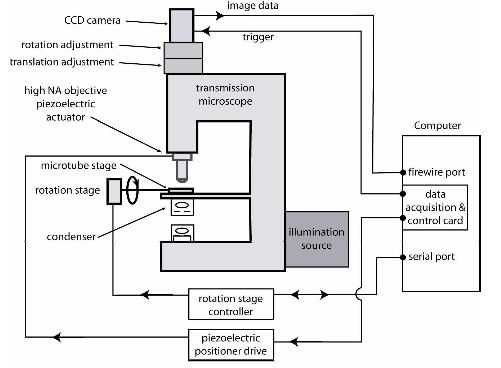
\includegraphics[scale=0.8]{Fauver_2005_setup.jpg}
\caption{OPT microscope for imaging single cell nuclei. A microcapillary tube injected with cells is rotated to sub-micron precision with refractive index matching  to 0.02. The piezoelectric objective lens is scanned axially to create extended depth of field images (figure from \cite{Fauver:2005}).}
\label{fig:fauver_setup}
\end{figure}







Wang and Wang report an improvement to OPT giving higher axial and lateral resolution even for slices far from the optical axis. \cite{Wang:2006hy, Wang:2007} As previously mentioned, to obtain high quality reconstructions the projections should closely approximate a line integral of parallel rays passing through the sample. \cite{Wang:2006hy} This is not exactly the case for  OPT which limits the resolution possible. Wang proposed placing an iris at the back focus of the objective lens. This reduces divergence of the projection rays from paths parallel to the optical axis.
Resolution 40$\mu$m in 2006. For 2007 system with NA of 0.014 resolution of 25$\mu$m is achieved.
(Also covers technique for placing iris in eOPT, mention and discuss in Section~\ref{subsec:eOPT}.)\textbf{Finish}


%\section{here}
Live specimen OPT not a topic taken up by many other groups due to difficulties in keeping specimen alive, problems with OCA, can only image very small specimen anyway. \cite{Boot:2008dt} Boot and Sharpe 2008.
Colas and Sharpe do live, time-lapse OPT in 2009, not particularly useful. Poor resolution due to lack of clearing \cite{Colas:2009}  


Computational methods for improving reconstructions in OPT by Birk in 2011 \cite{Birk:2011}






\subsection{Fluorescent OPT/emission OptCT}
\label{subsec:eOPT}

There are many optical stains which are fluorescent which meant the development of fluorescent or emission OptCT/OPT very useful for the study of biological specimen. REF


Walls 2005 - first mention of eOPT? Correction of artefacts. \cite{Walls:2005ja}

Oldham has dual set-up. However, it was not originally quantitative. Just pretty pictures. Steps by various groups to get quantitative information out of emission. What is the change to the set-up? \cite{Oldham:2006dfa}
quantitative: \cite{Kim:2008eua}


Imperial group investigating Opt combined with FRET and FLIM. Define these and some uses for the combined modality. What physical/software changes needed for this imaging.
FLIM OPT: \cite{McGinty:2008ix}, In vivo FLIM OPT \cite{McGinty:2011vm}.


Resolution improvement to eOPT in 2007 by Walls \cite{Walls:2007jl} is this quantitative?


Lorbeer - SLOT \cite{Lorbeer:2011}

\newpage
\section{Optical Clearing}
\label{sec:clearing}

%Need for refractive index matching to ensure parallel beam assumption is true enough that we can emloy traditional reconstruction techniques. 



\section{Optical Staining}
Sharpe 2002 stains for gene expression and limb bud growth. 

Discuss which stains are relevant for cancer biomarkers. \cite{Hanahan:2011gua}

Being able to use optical stains is extremely useful for computer recognition of organs, can pick better thresholds. \cite{Sharpe:2003cm}

Soufan 2003 \cite{Soufan:2003cd} gene expression during cardiac development. 
Highlights problem of whole-mount staining not working for all stains. Depends on size of specimen. Therefore, they took slices of embryo heart.


\section{Recent Research}
 Time gated OPT Bassi 2010 \cite{Bassi:2010}
 
 CLAHE Hornblad 2011 \cite{Hornblad:2011fh}


\bibliography{bibliography2}

\end{document}